\documentclass{beamer}
\usepackage{ctex}
\usepackage[export]{adjustbox}
\usepackage{listings}
\usepackage{xcolor}

\usetheme{focus}

\definecolor{codegreen}{RGB}{50 200 50}
\definecolor{codeblue}{RGB}{50 50 200}
\definecolor{codered}{RGB}{200 50 50}
\tikzset{
    global scale/.style={scale=#1,every node/.append style={scale=#1}},
    CC1/.style ={circle,minimum width = 30pt, minimum height =30pt, draw=black},
    CC2/.style ={circle,minimum width = 30pt, minimum height =30pt, draw=black, fill=blue!20},
    RA1/.style ={rectangle,minimum width = 30pt, minimum height =20pt, draw=black},
    RA2/.style ={rectangle,minimum width = 1cm, minimum height = 1cm, draw=black}
}

\title{算法分析与设计II}
\subtitle{2022-2023-2}
\date{Last Modified: 2023.1.16}
\institute{\vspace{2em} 数学与计算机学院 \\ 数据科学与大数据技术}
\titlegraphic{\vspace{5em} 
\includegraphics[scale=0.3]{fig/jlnu.pdf}}

\lstset{
    columns=flexible,       
    numbers=left,  
    numberstyle=\footnotesize\color{darkgray},  
    frame=shadowbox, 
    rulesepcolor= \color{gray}, 
    keywordstyle=\color{codeblue},         
    commentstyle=\color{codegreen},  
    stringstyle=\color{codered}, 
    showstringspaces=false,  
    xleftmargin=3em,
    xrightmargin=1em,              
    language=c++                           
}

\tikzset{
    CC1/.style ={
    circle,
    minimum width = 30pt, 
    minimum height =30pt, 
    draw=black
    }
}

\begin{document}
\frame{\titlepage}
\section{6. 高级数据结构}
\begin{frame}{6.1 并查集}
    \begin{itemize}
        \item \textcolor{blue}{不相交集合数据结构}(Disjoint Set) :将编号分别为$1…n$的$n$个对象划分为不相交集合,在每个集合中,选择其中某个元素$x$代表所在集合
        \item 基本操作:
        \begin{itemize}
            \item MAKE-SET(x) 	建立新的集合,唯一成员$x$
            \item UNION(x,y) 	将包含$x$和$y$的两个集合合并成一个新的集合
            \item FIND(x) 		返回指针,指向包含$x$的集合的\textcolor{blue}{“代表”}(representative)
        \end{itemize}
        \item 由于两个基本操作是\textcolor{blue}{UNION}(合并)和\textcolor{blue}{FIND}(查找),所以称为“并查集”
    \end{itemize}
\end{frame}
\begin{frame}{实现}
    \begin{itemize}
        \item 使用树的数据结构来表示并查集,在程序实现起来相对简单,森林中的每棵树作为一个集合,树的节点表示集合中的元素,树的根用来作为该集合的“代表”
        \begin{itemize}
            \item 查找操作相当于对树进行遍历,从某个节点沿着父节点指针找到这棵树的根节点
            \item 合并操作相当于两棵树合并成一棵树,两个节点位于两棵不同的树的时候,将一个节点所在树的根的父亲节点指向另一个节点所在树的根
        \end{itemize}
        \item 在具体程序实现中,使用一维数组p来实现,数组下标i表示每个节点,p[i]为指向其父节点的指针,即p[x]=y表示x的父节点为y
        \item p的初始值有两种设置方法,一种是均设为-1,另一种是令p[i]=i,两种方式在判断是否查找到树根有所不同,设成-1还有一个用处,可以用它来统计集合成员的数量
    \end{itemize}
\end{frame}
\begin{frame}{无向图的连通分量}
    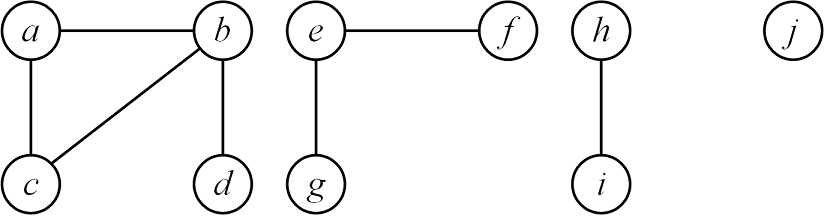
\includegraphics[width=0.7\textwidth,center]{fig/6-1.png}
    \begin{table}
        \begin{tabular}{c|c|c|c|c|c|c|c|c|c|c}
            边   & \multicolumn{10}{c}{构成的不相交集合} \\\hline
            初始     & \{a\}         & \{b\}   & \{c\}  & \{d\}  & \{e\}     & \{f\}  & \{g\}  & \{h\}   & \{i\}  & \{j\}  \\\hline
            (b,d)   & \{a\}         & \{b,d\} & \{c\}  & \{d\}  & \{e\}     & \{f\}  & \{g\}  & \{h\}   & \{i\}  & \{j\}   \\\hline
            (e,g)   & \{a\}         & \{b,d\} & \{c\}  &      & \{e,g\}   & \{f\}  &      & \{h\}   & \{i\}  & \{j\}   \\\hline
            (a,c)   & \{a,c\}        & \{b,d\} &      &      & \{e,g\}   & \{f\}  &      & \{h\}   & \{i\}  & \{j\}   \\\hline
            (h,i)   & \{a,c\}        & \{b,d\} &      &      & \{e,g\}   & \{f\}  &      & \{h,i\} &      & \{j\}   \\\hline
            (a,b)   & \{a,b,c,d\}    &       &      &      & \{e,g\}   & \{f\}  &      & \{h,i\} &      & \{j\}   \\\hline
            (e,f)   & \{a,b,c,d\}    &       &      &      & \{e,f,g\} &      &      & \{h,i\} &      & \{j\}   \\\hline
            (b,c)   & \{a,b,c,d\}    &       &      &      & \{e,f,g\} &      &      & \{h,i\} &      & \{j\}   \\\hline
        \end{tabular}
    \end{table}
\end{frame}
\begin{itemize}
    \item \textcolor{blue}{按秩合并}(union by rank)
    \begin{itemize}
        \item 增加一个Rank数组(初始值为0)来记录树的深度,也就是\textcolor{blue}{秩}
        \item 将秩较小的树的根指向秩较大的树的根
        \item 任意顺序的合并操作以后,包含$k$个节点的树的最大高度不超过$\log k$
    \end{itemize} 
\end{itemize}
\begin{lstlisting}
    void Union(int x,int y)  
    {   x = Find(x);
        y = Find(y);
        if(x==y) return;
        if(Rank[x] < Rank[y])
            p[x]=y;
        else {
            p[y]=x;
            if(Rank[x]==Rank[y])
                Rank[x]++;
        }
    }
\end{lstlisting}
    
\vspace*{3ex}
\begin{itemize}
    \item \textcolor{blue}{路径压缩}(path compression)
    \begin{itemize}
        \item 每次查找的时候,可以将查找路径上的节点修改成指向根节点,以便下次查找的时候速度更快
        \item 路径压缩的效果如图所示,(a)为压缩前,(b)为压缩后
    \end{itemize} 
\end{itemize}
\begin{columns}
    \column{0.6\textwidth}
    \begin{lstlisting}
    int Find(int x)
    {
        if(p[x] < 0)
            return x;
        p[x] = Find(p[x]);
        return p[x];
    }
    \end{lstlisting}
    \column{0.4\textwidth}
    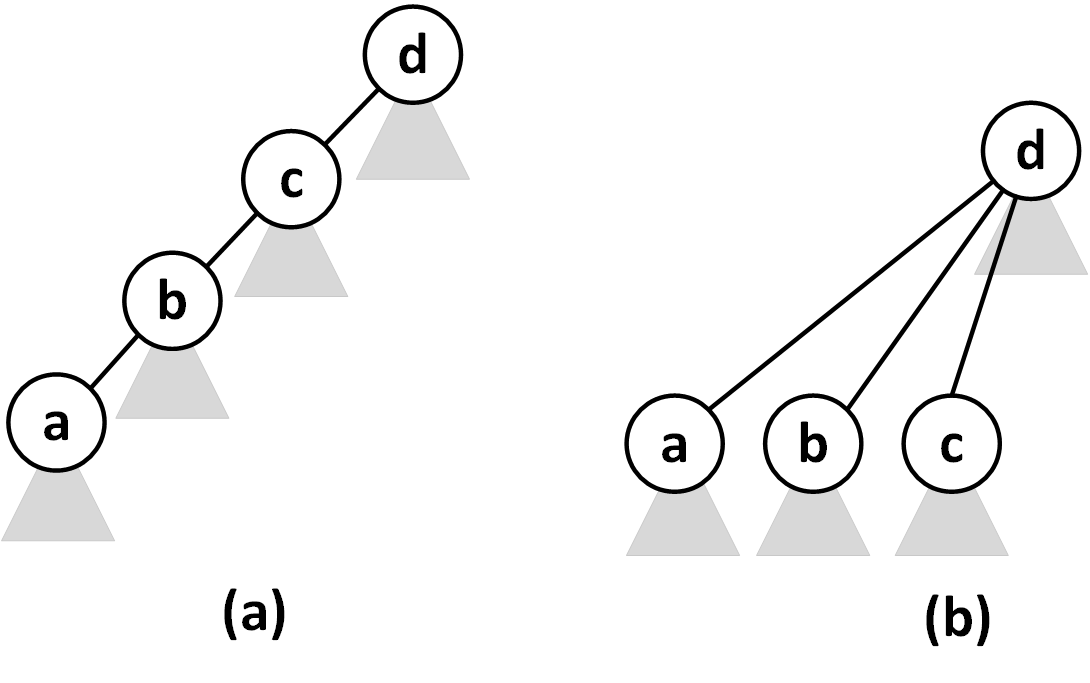
\includegraphics[width=\textwidth,right]{fig/6-2.png}
\end{columns}
\begin{frame}{2524 -- Ubiquitous Religions (poj.org)}
    \begin{itemize}
        \item $n$个学生信仰不同的宗教
        \vfill
        \item 给出$m$条信息,每条信息包含两个学生的编号,这两个学生信仰同一宗教
        \vfill
        \item 要求判断共有多少种宗教
    \end{itemize}
\end{frame}
\begin{frame}{6.2 线段树}
    \begin{itemize}
        \item \textcolor{blue}{线段树}(Segment tree) 使用二叉树的结构,每个节点表示一个包含起点和终点的区间,也可以看成是一个线段
        \vfill
        \item 线段树对区间信息进行存储,可以实现一些与区间计算有关的操作,例如区间最值问题、区间求和问题等,计算几何里面扫描线的操作也可以用线段树实现
        \vfill
        \item 由于线段树消耗大量存储空间,熟练掌握离散化处理方法十分重要
        \begin{block}{“在线” 与“离线”}
            \scriptsize{
                \quad 在程序设计过程中,如果开始时不需要知道所有输入,而是以序列的方式依次处理问题的算法,随着查询操作,数据也在实时变化,也称为“在线”查询,相应的算法称为\textcolor{blue}{在线算法},例如插入排序算法、贪心算法等\\
                \quad 相对的,开始时就需要知道问题的所有数据,每次查询操作时的数据保持不变,称为“离线”查询,相应的算法称为\textcolor{blue}{离线算法}。基于线段树的区间查询算法是离线查询,在多次查询的问题中能够提高效率}
        \end{block}
    \end{itemize}
\end{frame}
\begin{frame}{2182 -- Lost Cows (poj.org)}
    \begin{itemize}
        \item  $n$头牛编号为$1…n$,打乱顺序排成一列,除去队首的牛之外,给出每头牛在队列中前面编号比它小的牛的数量$k$,求队列中每头牛的编号
    \end{itemize}
    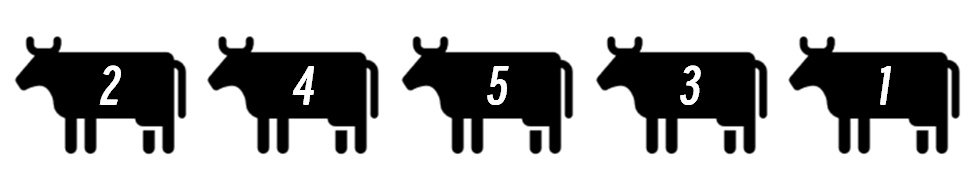
\includegraphics[width=0.8\textwidth,center]{fig/6-3.png}
    \begin{itemize}
        \item  维护一个线段树来解决该问题,创建一个线段树$T$,树中每个节点有3个属性$[p,r,n]$,分别代表线段左端点、线段右端点、左右端点之间节点的数量
    \end{itemize}
\end{frame}
\begin{frame}{构造线段树$(n=5)$}
    \begin{itemize}
        \item  从树根处依次比较:如果$k$小于等于左子树的$n$,则在左子树中继续查询;如果$k$大于左子树的$n$,则$k=k-n$,在右子树中继续查询;直到找到叶子节点($p=r$),此时的$p$即为要查询的编号
    \end{itemize}
    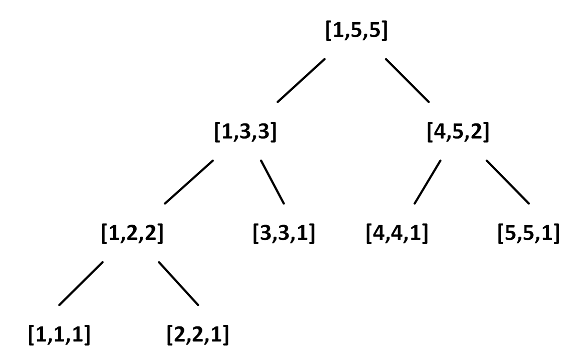
\includegraphics[width=0.8\textwidth,center]{fig/6-4.png}
\end{frame}
\begin{frame}{6.3 树状数组}
    \begin{itemize}
        \item \textcolor{blue}{树状数组}也称\textcolor{blue}{二元索引树}(Binary Indexed Tree)或\textcolor{blue}{Fenwick树}, 树状数组非常适合区间累计的计数与求和,尤其是多组查询,代码效率很高
        \item 与线段树相比,线段树可实现的功能更多,凡是树状数组能解决的问题,线段树同样可以解决
        \item 树状数组用一维数组C实现,每个元素代表不同区间(图中矩形横向范围)
        \begin{itemize}
            \item C[1]:[1-1],C[2]:[1-2],C[3]:[3-3],C[4]:[1-4],C[5]:[5-5],C[6]:[5-6],...
        \end{itemize}
    \end{itemize}
    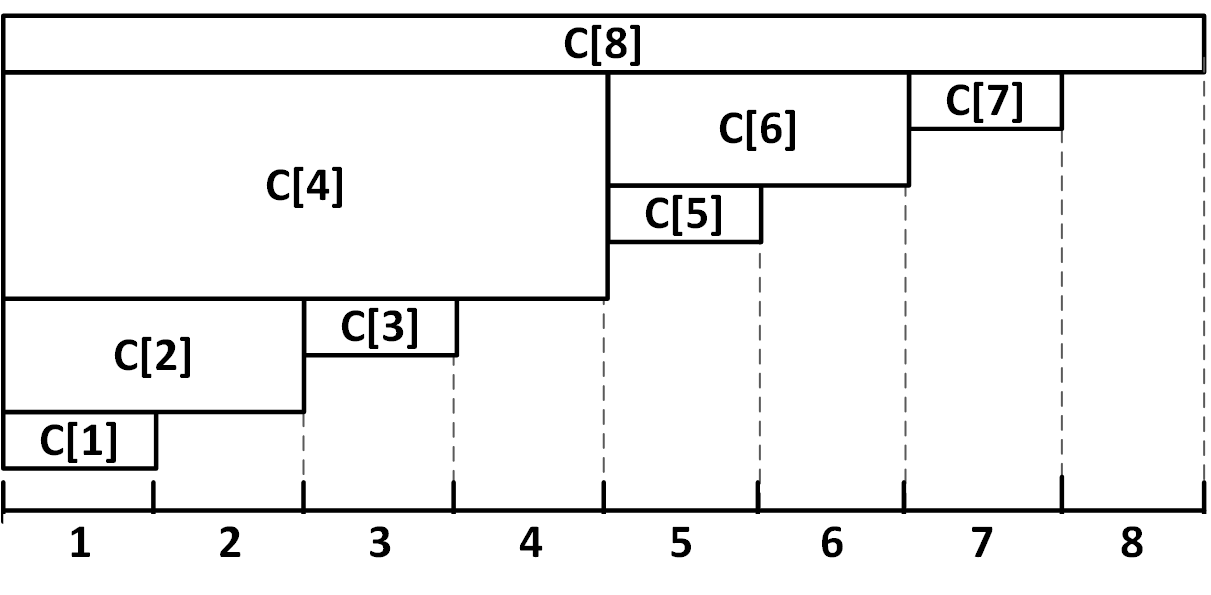
\includegraphics[width=0.7\textwidth,center]{fig/6-5.png}
\end{frame}
\begin{frame}{树状数组}
    \begin{itemize}
        \item 区间用下面方法确定:
        \begin{itemize}
            \item 将下标用二进制表示出来,然后看末位有几个0,设0的个数为$k$,则它代表的区间就向前推$2^k-1$
            \item 例如:$6=(110)_2$,$k=1$,向前推$2^1-1=1$,所以表示的区间为[5-6]
        \end{itemize}
        \item 树状数组两个基本操作:
        \begin{enumerate}[(1)]
            \item 更新/添加元素$x$:将$x$对应“列”的C值更新
            \begin{itemize}
                \item 例如:$x=1$,需要将$C[1],C[2],C[4],C[8]\ldots$都更新
                \item 计数:对应位置加1
                \item 求和:对应位置加$x$
            \end{itemize}
            \item 区间求和:将对应区间“行”的C值相加
            \begin{itemize}
                \item 对于$[1\ldots n]$区间求和,只需将对应“行”的C值相加,例如
                $$\sum [1\ldots 7]=C[4]+C[6]+C[7]$$ 
                \item 对于$[m\ldots n]$区间求和,只需$\sum [1\ldots n]$减去$\sum [1\ldots m-1]$,例如
                $$\sum[3\ldots 5]=\sum [1…5]-\sum [1…2]=C[4]+C[5]-C[2]$$
            \end{itemize}
        \end{enumerate}
    \end{itemize}
\end{frame}
\begin{frame}{lowbit}
    \begin{itemize}
        \item 计算公式:$lowbit(x)=x\&(-x)$,例如:$lowbit(6)$
        \begin{table}
            \begin{tabular}{r|c}
                十进制 & 二进制(32位int类型)                    \\\hline
                6   & \texttt{00000000000000000000000000000110} \\\hline
                -6  & \texttt{11111111111111111111111111111010}\\\hline
                \&  & \texttt{00000000000000000000000000000010} \\\hline
            \end{tabular}
        \end{table}
        \item 计算出来的$lowbit$值见下表
        \begin{table}
            \begin{tabular}{r|cccccccc}
                x         & 1    & 2    & 3    & 4    & 5    & 6    & 7    & 8 \\\hline
				lowbit(x) & 1    & 2    & 1    & 4    & 1    & 2    & 1    & 8 \\\hline
            \end{tabular}
        \end{table}
        \item 观察树状数组的两个基本操作可以发现,下标的变化值为上一个下标的$lowbit$值
        \begin{enumerate}[(1)]
            \item “更新”的列的下标变化,例如1对应列C的下标为{1,2,4,8,…},变化值为$lowbit(1),lowbit(2),lowbit(4),\ldots$ 
            \item “求和”的行的下标变化,例如[1-7]对应行C的下标为{7,6,4},变化值为$lowbit(7),lowbit(6)$            
        \end{enumerate}
    \end{itemize}
\end{frame}
\begin{frame}{2352 -- Stars (poj.org)}
    \begin{itemize}
        \item  给出$n$个星星的坐标$(x,y)$,按$y$递增,$y$相等$x$递增的次序
        \item 一颗星星的level定义为所有$x$和$y$均不大于该星星坐标的星星的总数,如图所示,编号1…5的星星的level分别为0,1,2,1,3
        \item 依次输出level为0…n-1的星星个数,level为0的有1个,level为1的有2个,依次类推,所以输出1,2,1,1,0
    \end{itemize}
    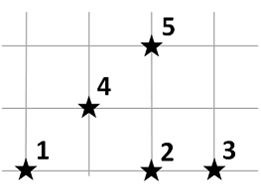
\includegraphics[width=0.4\textwidth,center]{fig/6-6.png}
    \begin{itemize}
        \item  本题中给出的星星坐标已经将$y$递增排序,统计每个星星$x$坐标之前有多少个星星即可,也就是每输入一个星星的坐标,level值就是[1…x-1]的累计值
    \end{itemize}
\end{frame}

\end{document}